\documentclass[14pt]{beamer}
\usetheme{Berkeley}
\usepackage[ngerman]{babel}
\usepackage[utf8]{inputenc}
\usepackage{graphicx}
\usepackage{pgfplots}
\usepackage{pgfplotstable}
\author{Bennet, Leonard, Jochen, Philip, Tim}
\title{Normalverteilung}
%\setbeamercovered{transparent} 
%\setbeamertemplate{navigation symbols}{} 
\logo{\includegraphics[scale=0.15]{logo_herder.png}} 
\institute{Herder Gymnasium Berlin} 
\date{}

\begin{document}

\begin{frame}
 \titlepage
\end{frame}


\section{Inhalt}
\begin{frame}{Inhalt}
 \begin{itemize}
 \item Standardisierung
 \item Die Integralfunktion
 \item Anwendung der Integralfunktion
\end{itemize} 
\end{frame}

\section{Standardisierung}

\begin{frame} {Standardisierung}

Standardisierung (auch Z-Transfomation) ist eine Transformation einer Zufallsvariable, z.B. X, sodass gilt: $$E(x) = \mu = 0$$ und $$V(x) = \sigma^2 = \sigma = 1$$

\end{frame}

\begin{frame} {Standardisierung}

Zunächste Erwartungswert auf Y-Achse verschieben:
$$ Z = X - \mu $$
Dann jede Verteilung auf eine Breite bringen
$$ Z = \frac{X - \mu}{\sigma} $$
Damit die Fläche gleichbleibt, gilt:
$$ Y = \sigma \cdot B_{n;p}(Z) $$

\end{frame}

\section{Die Integralfunktion}
\begin{frame} {Die Integralfunktion}

Die Integralfunktion soll liefern:
$$ \lim_{n \rightarrow \infty} P\left(\frac{X_n-n\cdotp}{\sqrt{n\cdotp\cdot(1-p)}} \le x\right) = \phi(x) $$

Allgemein geschrieben:
$$ \lim_{n \rightarrow \infty} P\left(\frac{X_n-\mu}{\sigma} \le x\right) = \phi(x) $$

\end{frame}

\begin{frame} {Die Integralfunktion}

Wie kann man das ausrechnen?

\end{frame}

\begin{frame} {Die Integralfunktion}

$$ \phi(x) = \int_{-\infty}^x \varphi(t)dt $$

\end{frame}

\begin{frame} {Die Integralfunktion}

Beweis:

 \begin{itemize}
  \item Aufsummieren von unendlich kleinen Spalten (da $n \rightarrow   \infty$)
  \item Genau dieser Grenzwert ist das Integral
  \item Daraus folgt: $ P(X \in ] \mu - n \cdot \sigma, \mu + n \cdot \sigma[) = \int_{-n}^{n}\varphi(t)dt $
 \end{itemize}

\end{frame}

\begin{frame} {Die Integralfunktion}

Beweis:

 \begin{itemize}
  \item Dann geht die untere Schranke nach $ - \infty $
  \item Die Formel ist dann: $ P(X \in ] -\infty, \mu + n \cdot \sigma[) = \int_{-\infty}^n\varphi(t)dt $
  \item Zudem ist $ X \in ]-\infty, \mu + n \cdot \sigma[ \Leftrightarrow X < \mu + n \cdot \sigma $
 \end{itemize}

\end{frame}

\begin{frame} {Die Integralfunktion}

 $$ X < \mu + n \cdot \sigma \Leftrightarrow $$ $$ X - \mu < n \cdot \sigma \Leftrightarrow $$ $$ \frac{X - \mu}{\sigma} < n \Leftrightarrow $$
 In der Funktion ist wird $ n \rightarrow x $ und $ X \rightarrow X_n $
 Das Ergebnis ist:
 $$ P\left(\frac{X_n - \mu}{\sigma}\right) = \int_{-\infty}^n\varphi(t)dt  $$

\end{frame}

\section{Anwendung der Integralfunktion}
\begin{frame} {Anwendung der Integralfunktion}

Beispiel:
\begin{itemize}
 \item p = 0,35
 \item n = 110
\end{itemize}

\end{frame}

\begin{frame} {Anwendung der Integralfunktion}

Beispiel:
\begin{itemize}
 \item p = 0,35
 \item n = 110
 \item $\mu = 0,35 \cdot 110 = 38,5 $
\end{itemize}

\end{frame}

\begin{frame} {Anwendung der Integralfunktion}

Beispiel:
\begin{itemize}
 \item p = 0,35
 \item n = 110
 \item $\mu = 0,35 \cdot 110 = 38,5 $
 \item $\sigma$ = $\sqrt{110 \cdot 0,35 \cdot 0,65}$ = $\sqrt{25,025} \approx 5$ 
\end{itemize}

\end{frame}

\begin{frame} {Anwendung der Integralfunktion}

Beispiel:
\begin{itemize}
 \item a) $P(X \le 45)$
 \item b) $P(X < 21)$
 \item c) $P(40 < X)$
 \item d) $P(45 < X_n \le 35)$
\end{itemize}

\end{frame}

\begin{frame} {Anwendung der Integralfunktion}

Beispiel a):
 
 $$P(X\le45)$$
 $$P(X_n \le 45) =  \phi\left(\frac{X_n - \mu}{\sigma}\right)$$
 $$ \phi(\frac{45 - 38,5}{5}) = \phi(1,3) $$

\end{frame}

\begin{frame} {Anwendung der Integralfunktion}
 
 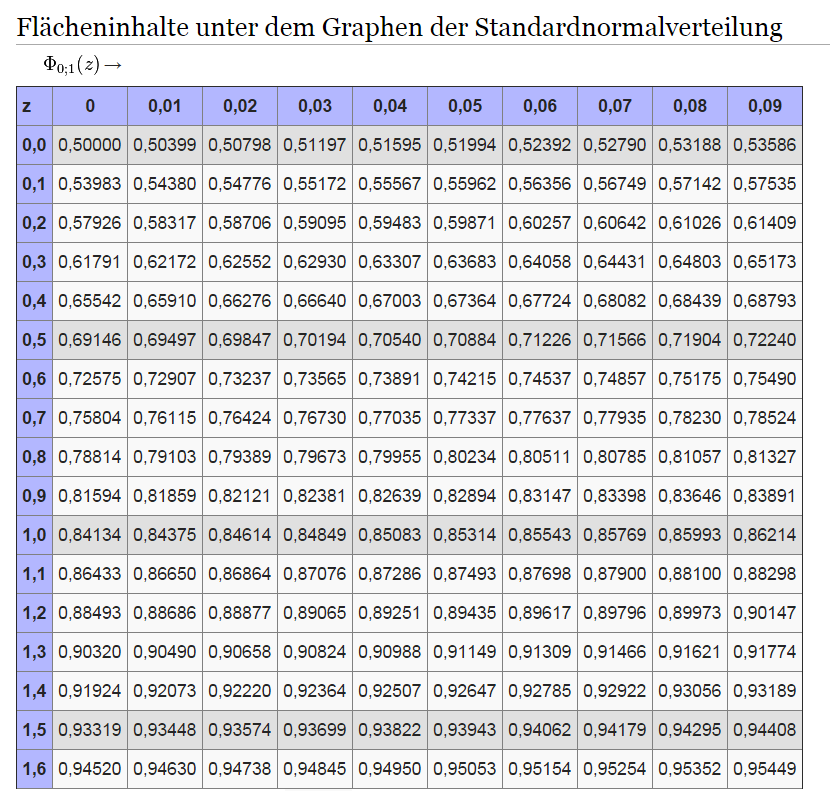
\includegraphics[width=7.0cm]{TabelleNormalverteilung.png}

\end{frame}
\begin{frame} {Anwendung der Integralfunktion}

Beispiel b):
 
 $$P(X_n < 21) \rightarrow P(X_n \le 20)$$
 $$P(X_n \le 20) =  \phi\left(\frac{X_n - \mu}{\sigma}\right)$$
 $$ \phi\left(\frac{20 - 38,5}{5}\right) = \phi(-3,7) $$
 
 Was nun?

\end{frame}
\begin{frame} {Anwendung der Integralfunktion}
 
 Es gilt:
 $$ \phi(x) = 1 - \phi(-x) $$

\end{frame}

\begin{frame} {Anwendung der Integralfunktion}
 
 $$P(X_n < 21) \rightarrow P(X_n \le 20)$$
 $$P(X_n \le 20) =  \phi\left(\frac{X_n - \mu}{\sigma}\right)$$
 $$ \phi\left(\frac{20 - 38,5}{5}\right) = \phi(-3,7) $$
 $$ \phi(-3,7) = 1 - \phi(3,7)$$

\end{frame}

\begin{frame} {Anwendung der Integralfunktion}
 
 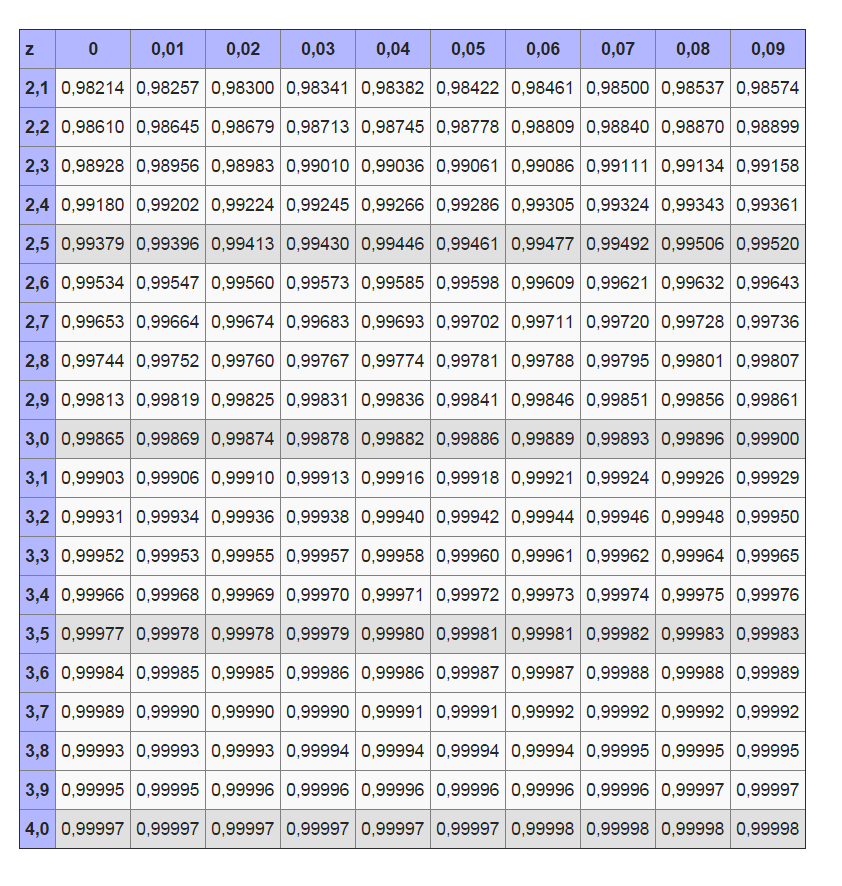
\includegraphics[width=7.0cm]{TabelleNormalverteilung2.png}

\end{frame}

\begin{frame} {Anwendung der Integralfunktion}

Beispiel c):
 
 $$P(40 < X_n)$$
 $1 - P(X_n \le 40)$
 Somit: $$P(X_n \le 40) =  \phi\left(\frac{X_n - \mu}{\sigma}\right)$$
 $$ \phi\left(\frac{40 - 38,5}{5}\right) = \phi(0,3) $$

\end{frame}

\begin{frame} {Anwendung der Integralfunktion}
 
 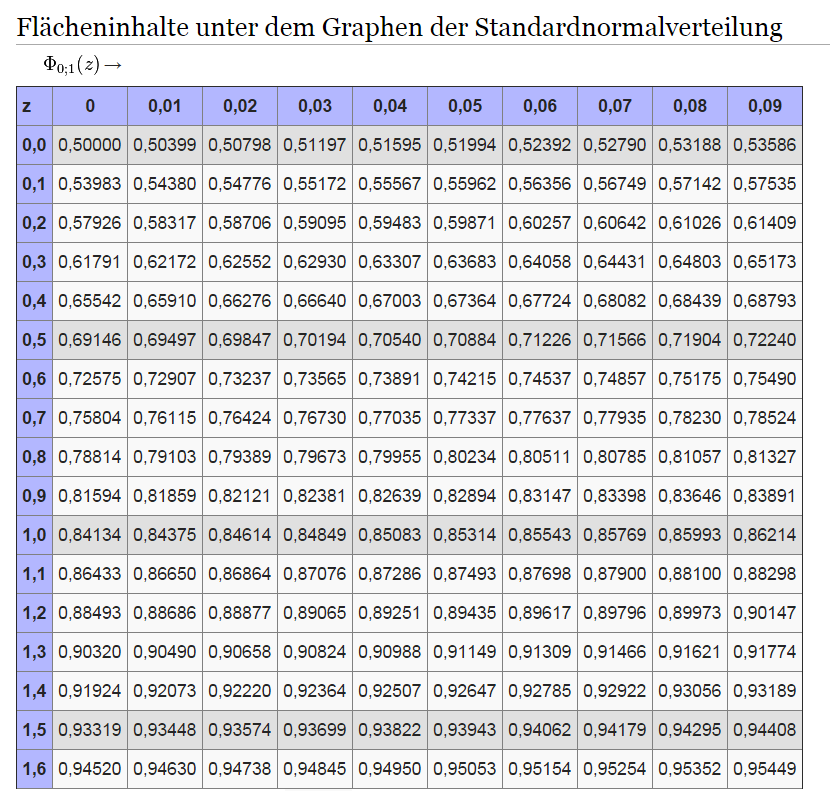
\includegraphics[width=7.0cm]{TabelleNormalverteilung.png}

\end{frame}

\begin{frame} {Anwendung der Integralfunktion}

Beispiel d):
 
 $$P(35 < X_n \le 45)$$
 $$P(X_n \le 45) - P(X_n \le 35)$$

\end{frame}

\begin{frame} {Anwendung der Integralfunktion}
 
 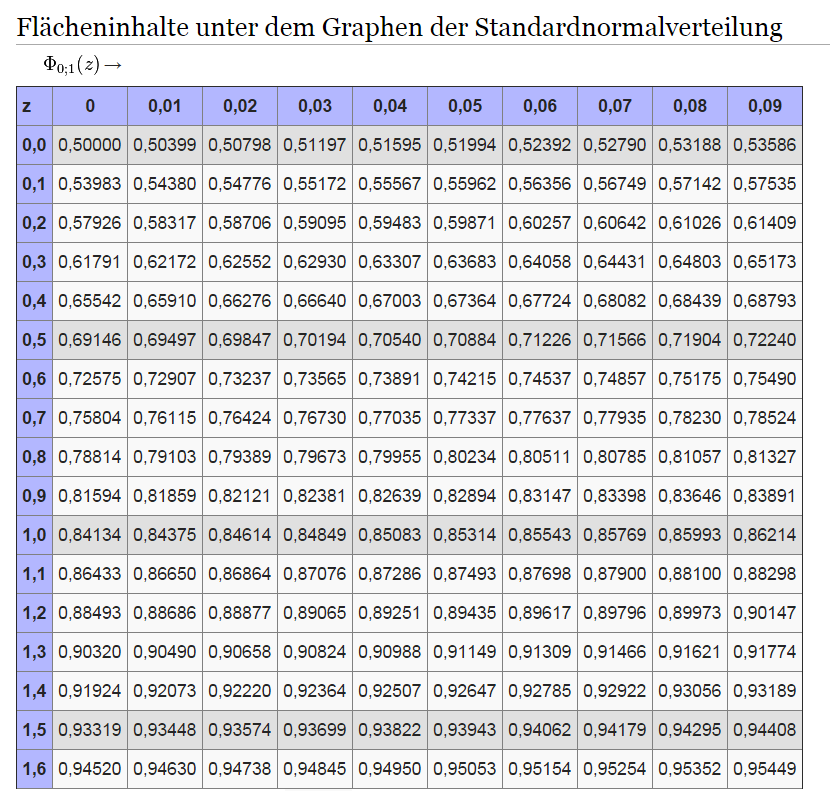
\includegraphics[width=7.0cm]{TabelleNormalverteilung.png}

\end{frame}

\section{k-$\sigma$-Intervalle}

\begin{frame}{k-$\sigma$-Intervalle}

Die Wahrscheinlichkeit ($P$), dass Ereignisse in einer k*$\sigma$-Umgebung liegen:
$ P(|X-p|\le k\cdot\sigma) = P(\mu-k\cdot\sigma\le X \le \mu + k\cdot\sigma)$\\
$ = P\left(\frac{\mu-k\cdot\sigma - \mu}{\sigma}\le \frac{X - \mu}{\sigma}\le \frac{\mu + k\cdot\sigma - \mu}{\sigma}\right)$\\
$ = P(-k \le Z \le k)$\\
$ \approx \phi(k) - \phi(-k)$\\
$ = \phi(k) - (1 - \phi(k))$\\
$ = \phi(k) + \phi(k) - 1$\\
$ = 2\phi(k)- 1$\\

\end{frame}

\begin{frame}{k-$\sigma$-Intervalle}

Das kann für $ k = {0;1;2;...}$ entsprechend eingesetzt werden.
 \\
Ergebnisse (Auswahl):
 \\
$ P(|X-p|\le \sigma) \approx 68,27$ \%\\
$ P(|X-p|\le 2\cdot\sigma) \approx 95,45$ \%\\
$ P(|X-p|\le 3\cdot\sigma) \approx 97,73$ \%

Vgl. Tschebyschow:

$ P(|X-p|\le 2\cdot\sigma) \approx 75$ \%\\
$ P(|X-p|\le 3\cdot\sigma) \approx 88$ \%\\

\end{frame}

\section{Vielen Dank!}
\begin{frame}{Vielen Dank!}
\begin{center}
\parskip 15pt
Vielen Dank für's Zuhören!
\end{center}
\end{frame}

\end{document}
